% ============================================================================
%  presentation.tex — Beamer Presentation
%  Projet : Architecture Kappa — Traitement Événementiel Unifié
%  Auteurs: Yazid TAHIRI ALAOUI, Souhayla ECH-CHARAY, Ouissal EL AMRANI
%  Compilation : pdflatex presentation.tex  (2 passes)
% ============================================================================
\documentclass[aspectratio=169, 12pt]{beamer}

% ── Encodage et langue ──────────────────────────────────────────────────────
\usepackage[utf8]{inputenc}
\usepackage[T1]{fontenc}
\usepackage[french]{babel}
\usepackage{lmodern}

% ── Paquets utilitaires ─────────────────────────────────────────────────────
\usepackage{graphicx}
\usepackage{booktabs}
\usepackage{tabularx}
\usepackage{array}
\usepackage{tikz}
\usetikzlibrary{shapes.geometric, arrows.meta, positioning, calc}
\usepackage{fontawesome5}

% ── Thème Beamer ────────────────────────────────────────────────────────────
\usetheme{Madrid}
\usecolortheme{default}

% ── Couleurs personnalisées (même palette que le rapport) ───────────────────
\definecolor{kappaBlue}{RGB}{0, 51, 102}
\definecolor{kappaGold}{RGB}{204, 153, 0}
\definecolor{kappaGreen}{RGB}{46, 139, 87}
\definecolor{kappaRed}{RGB}{200, 50, 50}
\definecolor{kappaBg}{RGB}{245, 247, 250}
\definecolor{kappaLightBlue}{RGB}{220, 235, 250}

\setbeamercolor{palette primary}{bg=kappaBlue, fg=white}
\setbeamercolor{palette secondary}{bg=kappaBlue!80, fg=white}
\setbeamercolor{palette tertiary}{bg=kappaBlue!60, fg=white}
\setbeamercolor{structure}{fg=kappaBlue}
\setbeamercolor{title}{fg=white, bg=kappaBlue}
\setbeamercolor{frametitle}{fg=kappaBlue, bg=kappaLightBlue}
\setbeamercolor{block title}{bg=kappaBlue, fg=white}
\setbeamercolor{block body}{bg=kappaLightBlue, fg=black}
\setbeamercolor{block title alerted}{bg=kappaRed, fg=white}
\setbeamercolor{block body alerted}{bg=red!5, fg=black}
\setbeamercolor{block title example}{bg=kappaGreen, fg=white}
\setbeamercolor{block body example}{bg=green!5, fg=black}
\setbeamercolor{item}{fg=kappaGold}

% ── Polices ─────────────────────────────────────────────────────────────────
\setbeamerfont{title}{size=\LARGE, series=\bfseries}
\setbeamerfont{frametitle}{size=\large, series=\bfseries}

% ── Barre de navigation et numérotation ─────────────────────────────────────
\setbeamertemplate{navigation symbols}{}
\setbeamertemplate{footline}{%
  \leavevmode%
  \hbox{%
    \begin{beamercolorbox}[wd=.33\paperwidth,ht=2.5ex,dp=1ex,center]{palette primary}%
      \usebeamerfont{author in head/foot}\insertshortauthor
    \end{beamercolorbox}%
    \begin{beamercolorbox}[wd=.34\paperwidth,ht=2.5ex,dp=1ex,center]{palette secondary}%
      \usebeamerfont{title in head/foot}\insertshorttitle
    \end{beamercolorbox}%
    \begin{beamercolorbox}[wd=.33\paperwidth,ht=2.5ex,dp=1ex,right]{palette tertiary}%
      \insertframenumber{} / \inserttotalframenumber\hspace*{2ex}
    \end{beamercolorbox}%
  }%
}

% ── Colonnes de tableau personnalisées ──────────────────────────────────────
\newcolumntype{L}[1]{>{\raggedright\arraybackslash}p{#1}}
\newcolumntype{C}[1]{>{\centering\arraybackslash}p{#1}}

% ── Métadonnées ─────────────────────────────────────────────────────────────
\title[Architecture Kappa]{Implémentation d'une Architecture Kappa}
\subtitle{Traitement événementiel unifié pour le e-commerce}
\author[Yazid, Souhayla, Ouissal]{%
  Yazid TAHIRI ALAOUI \and Souhayla ECH-CHARAY \and Ouissal EL AMRANI}
\institute[ENSAH]{%
  École Nationale des Sciences Appliquées d'Al Hoceima\\
  \textit{Gestion de Projets Informatiques} — Pr. Redouan ABAKOUY}
\date{Année universitaire 2025 -- 2026}
\titlegraphic{%
  
\includegraphics[height=1cm]{logos/UAE.png}\hspace{1.5cm}%
  
\includegraphics[height=1cm]{logos/ENSAH.png}%
}

% ============================================================================
\begin{document}

% ╔══════════════════════════════════════════════════════════════════════════╗
% ║  PAGE DE TITRE                                                         ║
% ╚══════════════════════════════════════════════════════════════════════════╝
\begin{frame}[plain]
  \titlepage
\end{frame}

% ╔══════════════════════════════════════════════════════════════════════════╗
% ║  PLAN                                                                  ║
% ╚══════════════════════════════════════════════════════════════════════════╝
\begin{frame}{Plan de la présentation}
  \tableofcontents
\end{frame}

% ════════════════════════════════════════════════════════════════════════════
%  SECTION 1 — INTRODUCTION
% ════════════════════════════════════════════════════════════════════════════
\section{Introduction et Contexte}

\begin{frame}{Contexte du projet}
  \begin{columns}[T]
    \begin{column}{0.55\textwidth}
      \begin{block}{Plateforme e-commerce fictive}
        \begin{itemize}
          \item Des milliers de clics, vues et achats chaque seconde
          \item Le Marketing veut des \textbf{statistiques en temps réel}
          \item Besoin d'alertes immédiates en cas d'\textbf{abandon de panier}
        \end{itemize}
      \end{block}
      \vspace{0.3cm}
      \begin{alertblock}{Problématique}
        Comment traiter un flux continu d'événements avec un \textbf{seul système unifié}, tout en garantissant la \textbf{cohérence} des résultats~?
      \end{alertblock}
    \end{column}
    \begin{column}{0.42\textwidth}
      \centering
      \begin{tikzpicture}[
        box/.style={rectangle, draw=kappaBlue, fill=kappaLightBlue, rounded corners, minimum width=3cm, minimum height=0.8cm, font=\small\bfseries},
        arr/.style={-{Stealth[length=3mm]}, thick, kappaBlue}
      ]
        \node[box] (sim) at (0,3) {Utilisateurs};
        \node[box, fill=kappaGold!20, draw=kappaGold] (kafka) at (0,1.8) {Apache Kafka};
        \node[box, fill=green!10, draw=kappaGreen] (proc) at (0,0.6) {Traitement Flux};
        \node[box] (res) at (0,-0.6) {Résultats};
        \draw[arr] (sim) -- (kafka);
        \draw[arr] (kafka) -- (proc);
        \draw[arr] (proc) -- (res);
      \end{tikzpicture}
    \end{column}
  \end{columns}
\end{frame}

% ════════════════════════════════════════════════════════════════════════════
%  SECTION 2 — ARCHITECTURE
% ════════════════════════════════════════════════════════════════════════════
\section{Architecture Kappa}

\begin{frame}{Lambda vs Kappa}
  \begin{columns}[T]
    \begin{column}{0.48\textwidth}
      \begin{alertblock}{\faTimesCircle\ Architecture Lambda (2011)}
        \begin{itemize}
          \item \textbf{2 couches} : Batch + Speed
          \item Code dupliqué (même logique × 2)
          \item Résultats potentiellement incohérents
          \item Maintenance complexe et coûteuse
        \end{itemize}
      \end{alertblock}
    \end{column}
    \begin{column}{0.48\textwidth}
      \begin{exampleblock}{\faCheckCircle\ Architecture Kappa (2014)}
        \begin{itemize}
          \item \textbf{1 seul flux} de traitement continu
          \item Code unique, pas de duplication
          \item Cohérence garantie par le \textbf{Replay}
          \item Simplicité opérationnelle
        \end{itemize}
      \end{exampleblock}
    \end{column}
  \end{columns}
  \vspace{0.4cm}
  \begin{block}{Pourquoi Kappa pour notre projet~?}
    \centering
    Les événements e-commerce sont \textbf{naturellement un flux continu}. Kappa est l'architecture la plus adaptée : simple, cohérente, temps réel.
  \end{block}
\end{frame}

\begin{frame}{Les 3 Piliers de l'Architecture Kappa}
  \begin{columns}[T]
    \begin{column}{0.32\textwidth}
      \begin{block}{\centering \faDatabase\\ Pilier 1\\Log d'Événements}
        \scriptsize
        \begin{itemize}
          \item Stockage \textbf{immuable} et ordonné
          \item Rétention configurable
          \item Permet le replay
          \item Technologie : \textbf{Apache Kafka}
        \end{itemize}
      \end{block}
    \end{column}
    \begin{column}{0.32\textwidth}
      \begin{block}{\centering \faCogs\\ Pilier 2\\Traitement de Flux}
        \scriptsize
        \begin{itemize}
          \item Traitement \textbf{en continu}
          \item Topologies spécialisées
          \item Chaîne de traitement
          \item Technologie : \textbf{Flink / Python}
        \end{itemize}
      \end{block}
    \end{column}
    \begin{column}{0.32\textwidth}
      \begin{block}{\centering \faRedo\\ Pilier 3\\Replay = Cohérence}
        \scriptsize
        \begin{itemize}
          \item Rejouer depuis le début
          \item Recalculer les résultats
          \item Remplace le batch layer
          \item Validation : \textbf{Replay = RT}
        \end{itemize}
      \end{block}
    \end{column}
  \end{columns}
  \vspace{0.4cm}
  \begin{block}{}
    \centering\small
    \textbf{Sans rétention} $\to$ pas de replay. \textbf{Sans replay} $\to$ pas de Kappa.
  \end{block}
\end{frame}

\begin{frame}{Notre pipeline Kappa}
  \centering
  \begin{tikzpicture}[
    box/.style={rectangle, draw=kappaBlue, fill=kappaLightBlue, rounded corners=4pt, minimum width=2.2cm, minimum height=1cm, text width=2cm, align=center, font=\scriptsize\bfseries},
    kafka/.style={rectangle, draw=kappaGold, fill=kappaGold!15, rounded corners=4pt, minimum width=2.2cm, minimum height=1cm, text width=2cm, align=center, font=\scriptsize\bfseries},
    arr/.style={-{Stealth[length=2.5mm]}, thick, kappaBlue!70}
  ]
    \node[box, fill=blue!10] (sim) at (0,0) {Simulateur\\[2pt]\tiny simulateur.py};
    \node[kafka] (k1) at (3,0) {Kafka\\[2pt]\tiny clics\_ecommerce};
    \node[box, fill=green!10, draw=kappaGreen] (filt) at (6,0) {Filtrage\\[2pt]\tiny filtrage.py};
    \node[kafka] (k2) at (9,0) {Kafka\\[2pt]\tiny clics\_filtres};
    \node[box, fill=orange!10, draw=orange] (agg) at (11.5,1.2) {Agrégation\\[2pt]\tiny agregation.py};
    \node[box, fill=red!10, draw=kappaRed] (det) at (11.5,-1.2) {Détection\\Abandon\\[2pt]\tiny detection.py};

    \draw[arr] (sim) -- (k1);
    \draw[arr] (k1) -- (filt);
    \draw[arr] (filt) -- (k2);
    \draw[arr] (k2) -- (agg);
    \draw[arr] (k2) -- (det);
  \end{tikzpicture}

  \vspace{0.5cm}
  \footnotesize
  \begin{tabular}{lccc}
    \toprule
    \textbf{Topic Kafka} & \textbf{Contenu} & \textbf{Rétention} & \textbf{Partitions} \\
    \midrule
    \texttt{clics\_ecommerce} & Événements bruts & 7 jours & 3 \\
    \texttt{clics\_filtres} & Événements nettoyés & 3 jours & 3 \\
    \texttt{stats\_produits} & Statistiques agrégées & 1 jour & 1 \\
    \texttt{alertes\_marketing} & Alertes abandon & 7 jours & 1 \\
    \bottomrule
  \end{tabular}
\end{frame}

\begin{frame}{Technologies utilisées}
  \centering
  \begin{tabular}{lll}
    \toprule
    \textbf{Technologie} & \textbf{Rôle} & \textbf{Version} \\
    \midrule
    \textcolor{kappaBlue}{\faStream}\ Apache Kafka & Log d'événements, rétention, distribution & 7.3.0 \\
    \textcolor{kappaBlue}{\faSitemap}\ Apache Zookeeper & Coordination du cluster Kafka & 7.3.0 \\
    \textcolor{kappaGreen}{\faBolt}\ Apache Flink & Moteur de traitement de flux & 1.17 \\
    \textcolor{kappaGold}{\faCode}\ Python & Simulation et topologies & 3.10+ \\
    \textcolor{kappaGold}{\faPuzzlePiece}\ kafka-python & Client Python pour Kafka & 2.3.x \\
    \textcolor{kappaBlue}{\faDocker}\ Docker \& Compose & Conteneurisation de l'infra & 29.x \\
    \bottomrule
  \end{tabular}
\end{frame}

% ════════════════════════════════════════════════════════════════════════════
%  SECTION 3 — ACTEURS
% ════════════════════════════════════════════════════════════════════════════
\section{Acteurs et Rôles}

\begin{frame}{Gouvernance : MOA / MOE / Chef de Projet}
  \begin{columns}[T]
    \begin{column}{0.32\textwidth}
      \begin{block}{\centering \faUsers\ MOA\\[-2pt]\scriptsize Maîtrise d'Ouvrage}
        \centering\small
        Équipe \textbf{Marketing}\\[4pt]
        \scriptsize
        \begin{itemize}
          \item Définit les besoins
          \item Valide les résultats
          \item Vérifie la recette
        \end{itemize}
      \end{block}
    \end{column}
    \begin{column}{0.32\textwidth}
      \begin{block}{\centering \faProjectDiagram\ Chef de Projet\\[-2pt]\scriptsize Coordinateur}
        \centering\small
        Lien MOA $\leftrightarrow$ MOE\\[4pt]
        \scriptsize
        \begin{itemize}
          \item Planifie les sprints
          \item Gère les risques
          \item Assure la communication
        \end{itemize}
      \end{block}
    \end{column}
    \begin{column}{0.32\textwidth}
      \begin{block}{\centering \faLaptopCode\ MOE\\[-2pt]\scriptsize Maîtrise d'Œuvre}
        \centering\small
        Équipe \textbf{Technique}\\[4pt]
        \scriptsize
        \begin{itemize}
          \item Conçoit l'architecture
          \item Développe le code
          \item Déploie l'infra
        \end{itemize}
      \end{block}
    \end{column}
  \end{columns}

  \vspace{0.5cm}
  \centering\small
  \begin{tabular}{lcc}
    \toprule
    \textbf{Membre} & \textbf{Rôle principal} \\
    \midrule
    Yazid TAHIRI ALAOUI & MOE — Développeur \\
    Souhayla ECH-CHARAY & Chef de Projet \\
    Ouissal EL AMRANI & MOA — Validation \\
    \bottomrule
  \end{tabular}
\end{frame}

\begin{frame}{Matrice RACI}
  \centering\footnotesize
  \begin{tabular}{L{4cm} C{2cm} C{2cm} C{2cm}}
    \toprule
    \textbf{Activité} & \textbf{MOA} & \textbf{Chef Projet} & \textbf{MOE} \\
    \midrule
    Définir les besoins & \textcolor{kappaBlue}{\textbf{R}} & C & I \\
    Choisir l'architecture & C & \textcolor{kappaGold}{\textbf{A}} & \textcolor{kappaBlue}{\textbf{R}} \\
    Planifier les sprints & I & \textcolor{kappaBlue}{\textbf{R}} & C \\
    Déployer l'infrastructure & I & I & \textcolor{kappaBlue}{\textbf{R}} \\
    Développer les topologies & I & C & \textcolor{kappaBlue}{\textbf{R}} \\
    Tester la cohérence & C & \textcolor{kappaGold}{\textbf{A}} & \textcolor{kappaBlue}{\textbf{R}} \\
    Valider les résultats & \textcolor{kappaBlue}{\textbf{R}} & A & I \\
    \bottomrule
  \end{tabular}
  \vspace{0.4cm}

  \small \textbf{R} = Responsable \quad \textbf{A} = Approbateur \quad \textbf{C} = Consulté \quad \textbf{I} = Informé
\end{frame}

% ════════════════════════════════════════════════════════════════════════════
%  SECTION 4 — PLANIFICATION
% ════════════════════════════════════════════════════════════════════════════
\section{Planification et Estimation}

\begin{frame}{Découpage en Sprints}
  \footnotesize
  \begin{tabular}{L{1.8cm} L{4.5cm} L{4cm} C{1cm} C{1cm}}
    \toprule
    \textbf{Sprint} & \textbf{Objectif} & \textbf{Livrable} & \textbf{Points} & \textbf{Statut} \\
    \midrule
    Sprint 0 & Cadrage \& Choix architecture & Document de décision & 3 & \textcolor{kappaGreen}{\faCheck} \\[4pt]
    Sprint 1 & Infrastructure Docker & Kafka + Flink opérationnels & 8 & \textcolor{kappaGreen}{\faCheck} \\[4pt]
    Sprint 2 & Simulateur + 3 Topologies & Pipeline fonctionnel & 13 & \textcolor{kappaGreen}{\faCheck} \\[4pt]
    Sprint 3 & Validation + Rapport & Test replay + documentation & 8 & \textcolor{kappaGreen}{\faCheck} \\
    \bottomrule
  \end{tabular}

  \vspace{0.4cm}
  \begin{exampleblock}{Estimation par Planning Poker}
    \small Méthode collaborative pour estimer les \textit{story points}. Permet d'éviter la sous-estimation, risque fréquent avec des technologies nouvelles (Kafka, Flink).
  \end{exampleblock}
\end{frame}

\begin{frame}{Diagramme de Gantt}
  \centering
  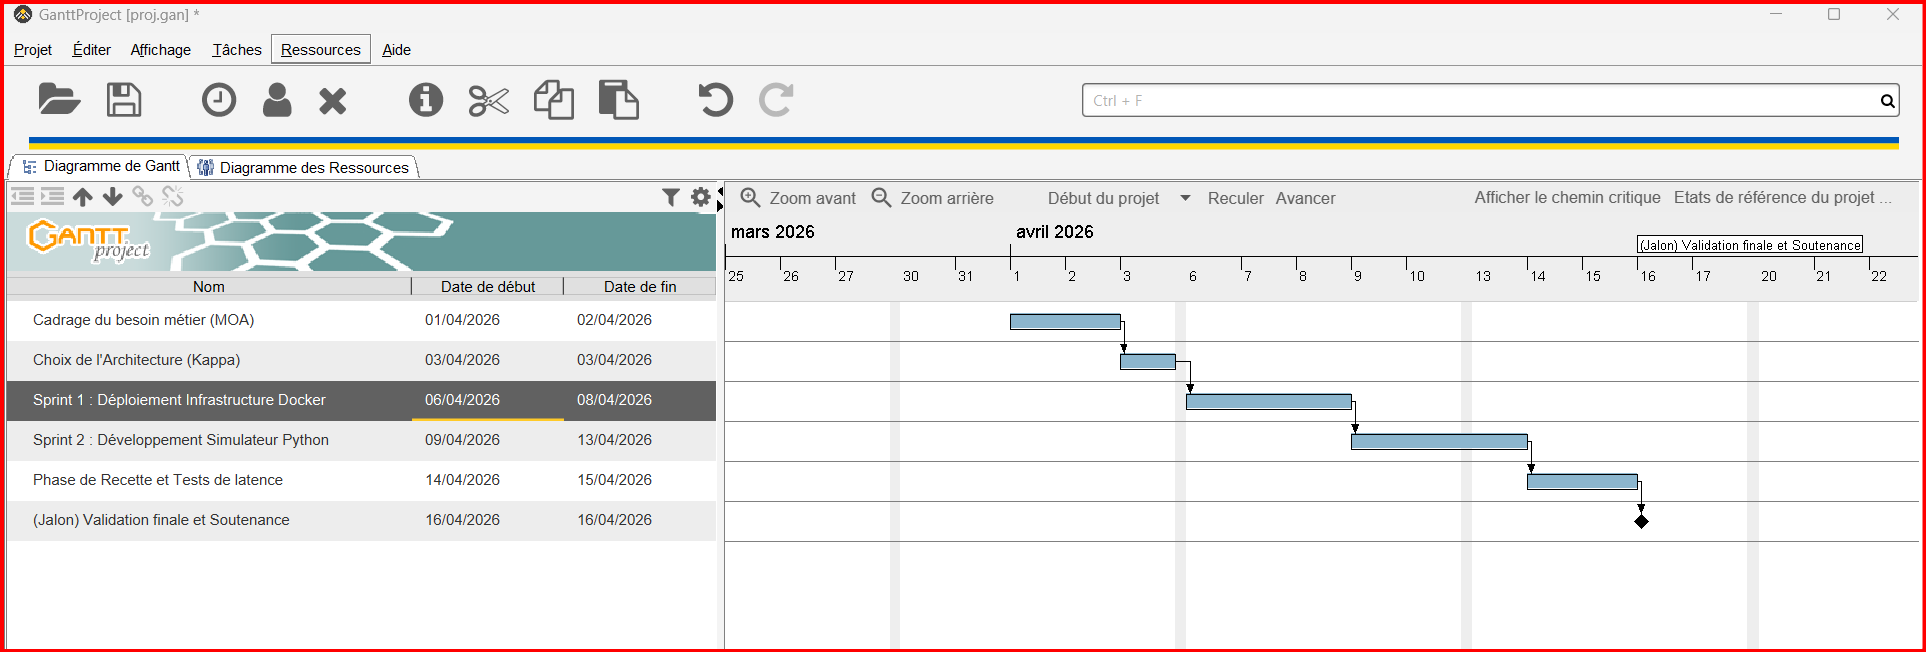
\includegraphics[width=\textwidth]{../screenshots/Gantt.png}
  \vspace{0.3cm}

  \small Planification temporelle réalisée avec \textbf{GanttProject}, permettant d'identifier le chemin critique du projet.
\end{frame}

\begin{frame}{User Stories \& Planning Poker}
  \footnotesize
  \begin{tabular}{L{5cm} C{2cm} C{2.5cm} C{1.5cm}}
    \toprule
    \textbf{User Story} & \textbf{Estim. initiale} & \textbf{Estim. consensus} & \textbf{Réel} \\
    \midrule
    US1 : Déployer Kafka & 3 & 5 & 5 \\
    US2 : Simulateur e-commerce & 2 & 3 & 3 \\
    US3 : Filtrage des bots & 3 & 3 & 3 \\
    US4 : Agrégation temps réel & 5 & 5 & 5 \\
    US5 : Détection abandon & 5 & 8 & 5 \\
    US6 : Test de replay & 3 & 3 & 3 \\
    \bottomrule
  \end{tabular}
  \vspace{0.3cm}
  \begin{block}{Leçon apprise}
    \small L'estimation initiale sous-estimait souvent la complexité. Le Planning Poker permet d'avoir des estimations plus réalistes grâce au \textbf{consensus de l'équipe}.
  \end{block}
\end{frame}

% ════════════════════════════════════════════════════════════════════════════
%  SECTION 5 — MÉTHODOLOGIE
% ════════════════════════════════════════════════════════════════════════════
\section{Méthodologie Agile}

\begin{frame}{Scrum \& Kanban}
  \begin{columns}[T]
    \begin{column}{0.48\textwidth}
      \begin{block}{\faSync\ Scrum}
        \begin{itemize}
          \item Itérations courtes (Sprints)
          \item Livraison incrémentale
          \item Feedback continu de la MOA
          \item Sprint Review en fin de sprint
          \item Rétrospective d'équipe
        \end{itemize}
      \end{block}
    \end{column}
    \begin{column}{0.48\textwidth}
      \begin{block}{\faColumns\ Kanban (Taiga)}
        \begin{itemize}
          \item Visualisation du flux de travail
          \item Colonnes : NEW $\to$ READY $\to$ IN PROGRESS $\to$ DONE
          \item Limite du travail en cours
          \item Amélioration continue
        \end{itemize}
      \end{block}
    \end{column}
  \end{columns}

  \vspace{0.4cm}
  \centering
  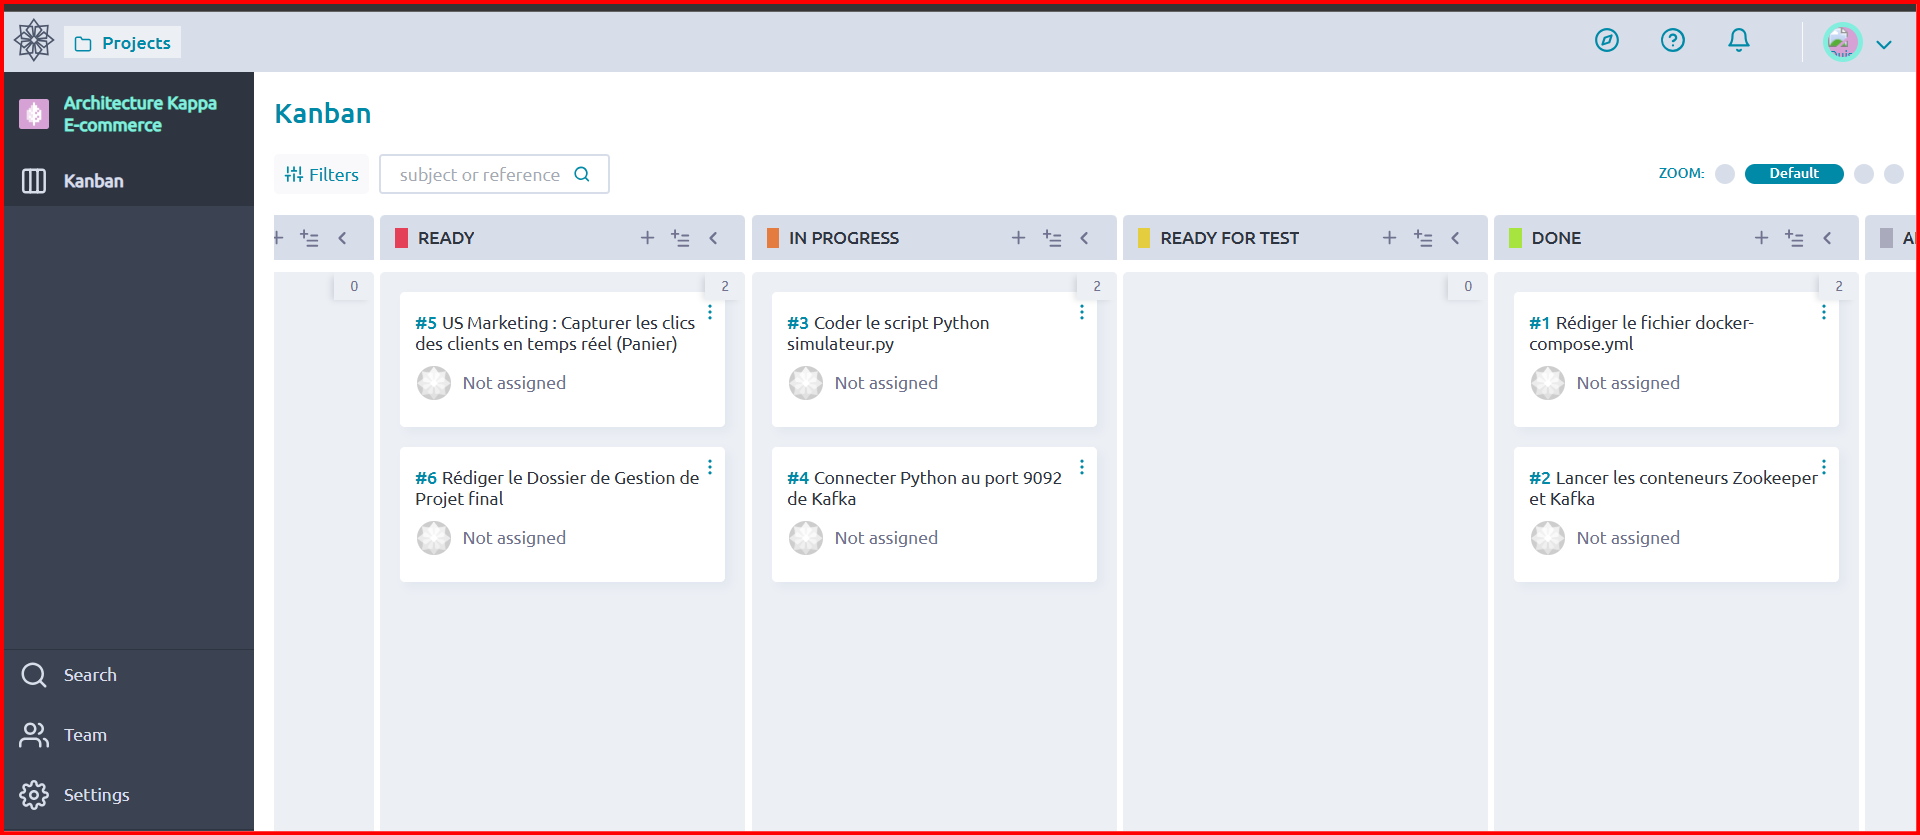
\includegraphics[width=0.85\textwidth]{../screenshots/taiga.png}
\end{frame}

% ════════════════════════════════════════════════════════════════════════════
%  SECTION 6 — IMPLÉMENTATION
% ════════════════════════════════════════════════════════════════════════════
\section{Implémentation Technique}

\begin{frame}{Infrastructure Docker}
  \begin{columns}[T]
    \begin{column}{0.45\textwidth}
      \begin{block}{Services déployés}
        \small
        \begin{tabular}{ll}
          \toprule
          \textbf{Service} & \textbf{Rôle} \\
          \midrule
          Zookeeper & Coordination \\
          Kafka & Log d'événements \\
          Flink JM & Gestion des jobs \\
          Flink TM & Exécution \\
          \bottomrule
        \end{tabular}
      \end{block}
      \vspace{0.2cm}
      \small Commande de lancement~:\\
      \texttt{docker-compose up -d}
    \end{column}
    \begin{column}{0.52\textwidth}
      \centering
      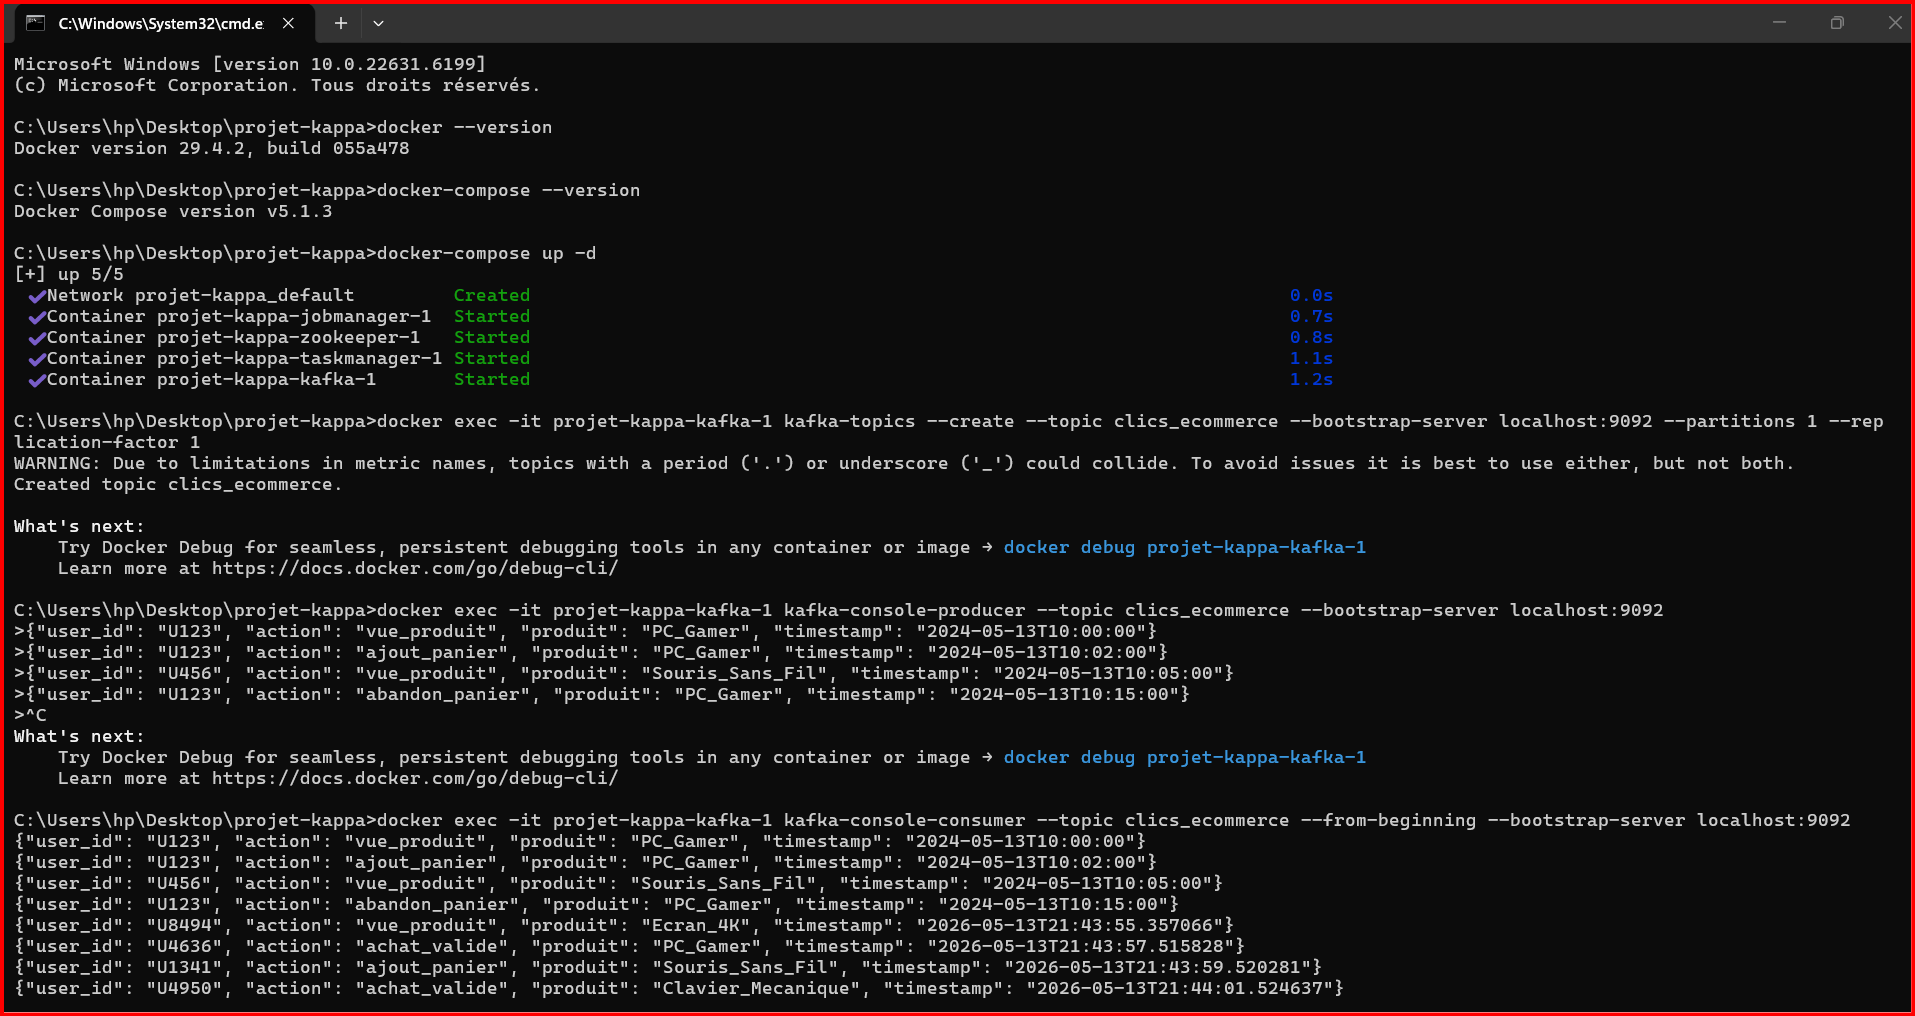
\includegraphics[width=\textwidth]{../screenshots/2.png}
    \end{column}
  \end{columns}
\end{frame}

\begin{frame}{Topologie 1 — Filtrage des bots}
  \begin{columns}[T]
    \begin{column}{0.40\textwidth}
      \begin{block}{Principe}
        \small
        \begin{itemize}
          \item $\sim$20\% du trafic web provient de robots
          \item Détection par : champ \texttt{is\_bot}, user-agent, préfixe \texttt{BOT\_}
          \item Événements humains $\to$ \texttt{clics\_filtres}
        \end{itemize}
      \end{block}
    \end{column}
    \begin{column}{0.57\textwidth}
      \centering
      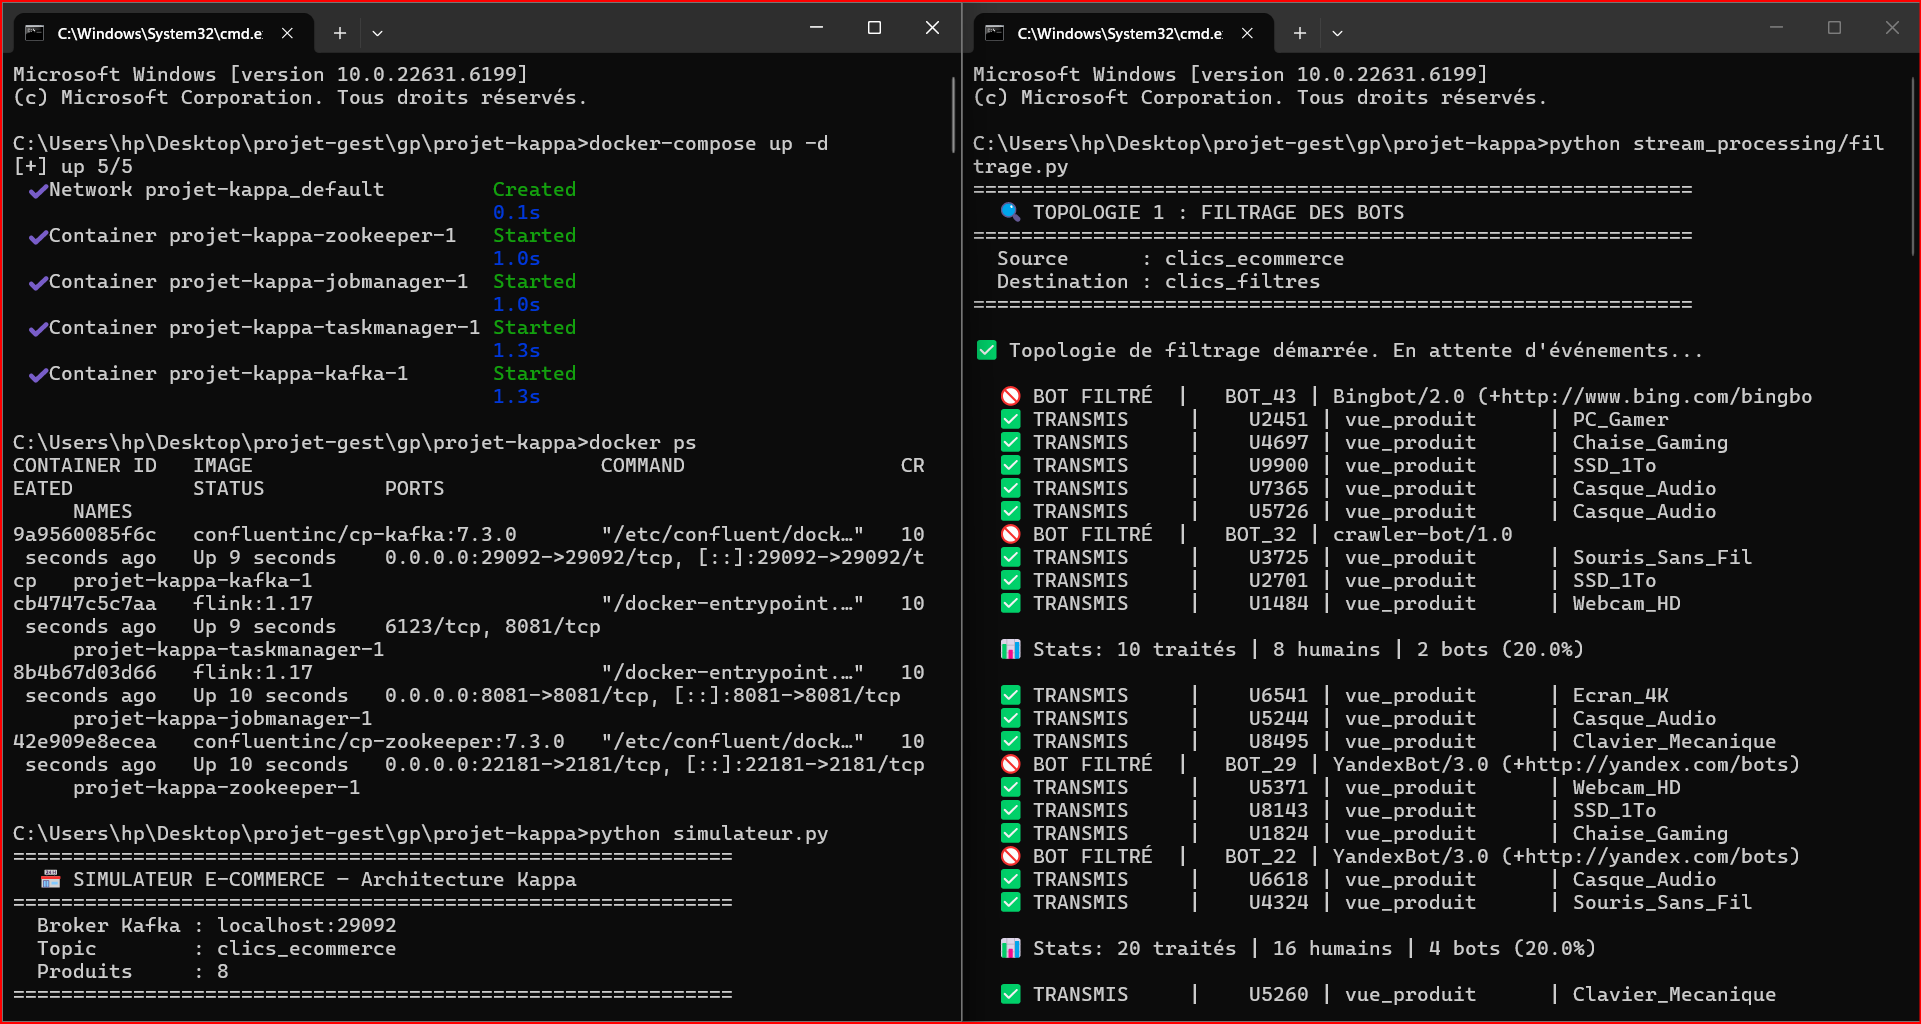
\includegraphics[width=\textwidth]{../screenshots/filtrage_bots.png}
    \end{column}
  \end{columns}
\end{frame}

\begin{frame}{Topologie 2 — Agrégation temps réel}
  \begin{columns}[T]
    \begin{column}{0.40\textwidth}
      \begin{block}{Métriques calculées}
        \small
        \begin{itemize}
          \item Vues par produit
          \item Ajouts panier
          \item Nombre d'achats
          \item Chiffre d'affaires (MAD)
          \item Taux de conversion
        \end{itemize}
      \end{block}
      \vspace{0.2cm}
      \small \textbf{Fenêtre :} 30 secondes glissantes
    \end{column}
    \begin{column}{0.57\textwidth}
      \centering
      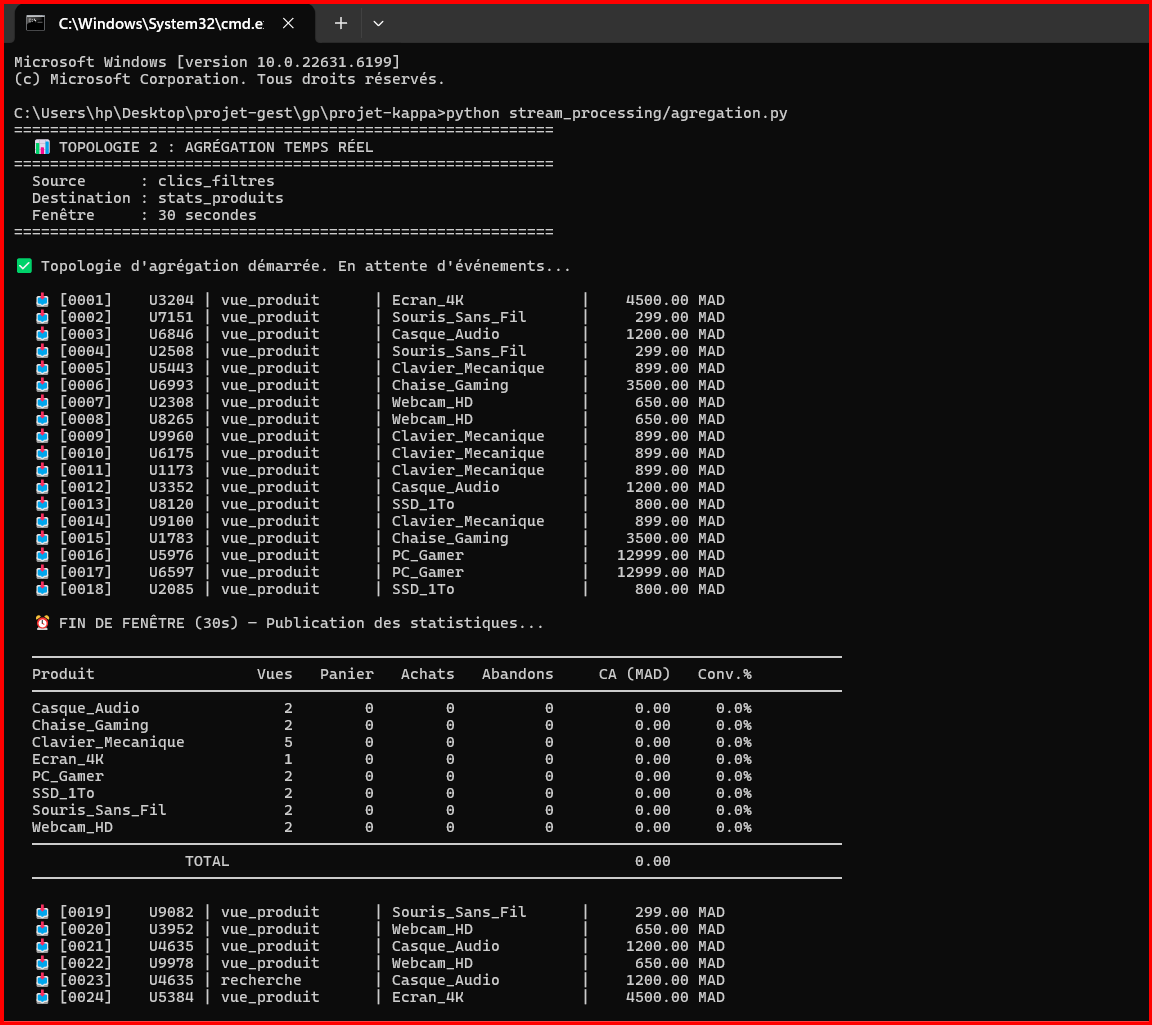
\includegraphics[width=\textwidth]{../screenshots/agregation_stats.png}
    \end{column}
  \end{columns}
\end{frame}

\begin{frame}{Topologie 3 — Détection d'abandon de panier}
  \begin{columns}[T]
    \begin{column}{0.40\textwidth}
      \begin{block}{Traitement avec état}
        \small
        \begin{itemize}
          \item \textbf{ajout\_panier} $\to$ Timer 60s
          \item \textbf{achat\_valide} $\to$ Timer annulé
          \item \textbf{Timeout} $\to$ Alerte marketing
        \end{itemize}
      \end{block}
      \vspace{0.2cm}
      \begin{exampleblock}{\small Règle métier}
        \scriptsize
        Prix $>$ 2000 MAD $\to$ Priorité \textbf{haute}\\
        Action : email de relance avec $-10\%$
      \end{exampleblock}
    \end{column}
    \begin{column}{0.57\textwidth}
      \centering
      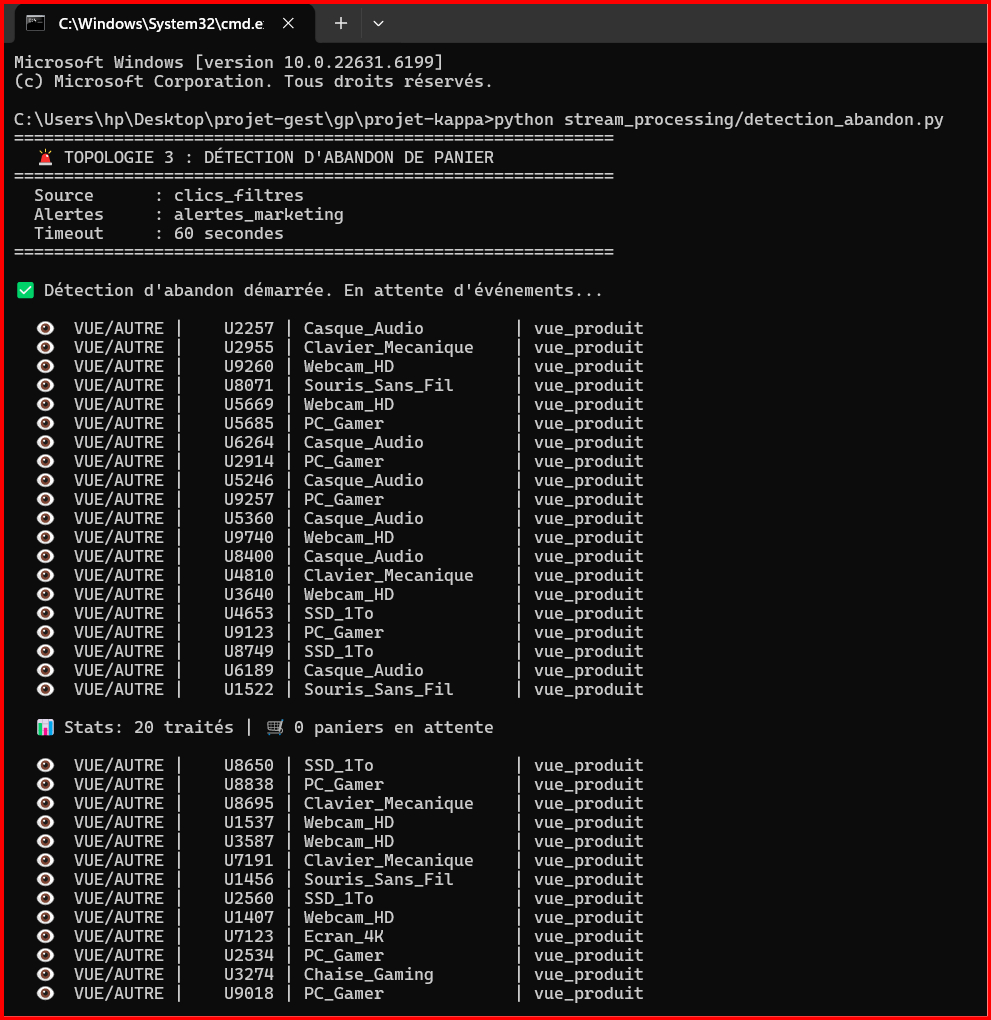
\includegraphics[width=\textwidth]{../screenshots/alerte_abandon1.png}
    \end{column}
  \end{columns}
\end{frame}

\begin{frame}{Rétention \& Replay — La preuve Kappa}
  \begin{block}{Le test fondamental de cohérence}
    \centering
    \small
    Rejouer \textbf{TOUS} les événements depuis le début $\to$ Recalculer les statistiques $\to$ Comparer avec le temps réel\\[6pt]
    \textcolor{kappaGreen}{\textbf{Si Replay = Temps Réel $\Rightarrow$ Le système est cohérent \faCheckCircle}}
  \end{block}

  \vspace{0.3cm}
  \centering
  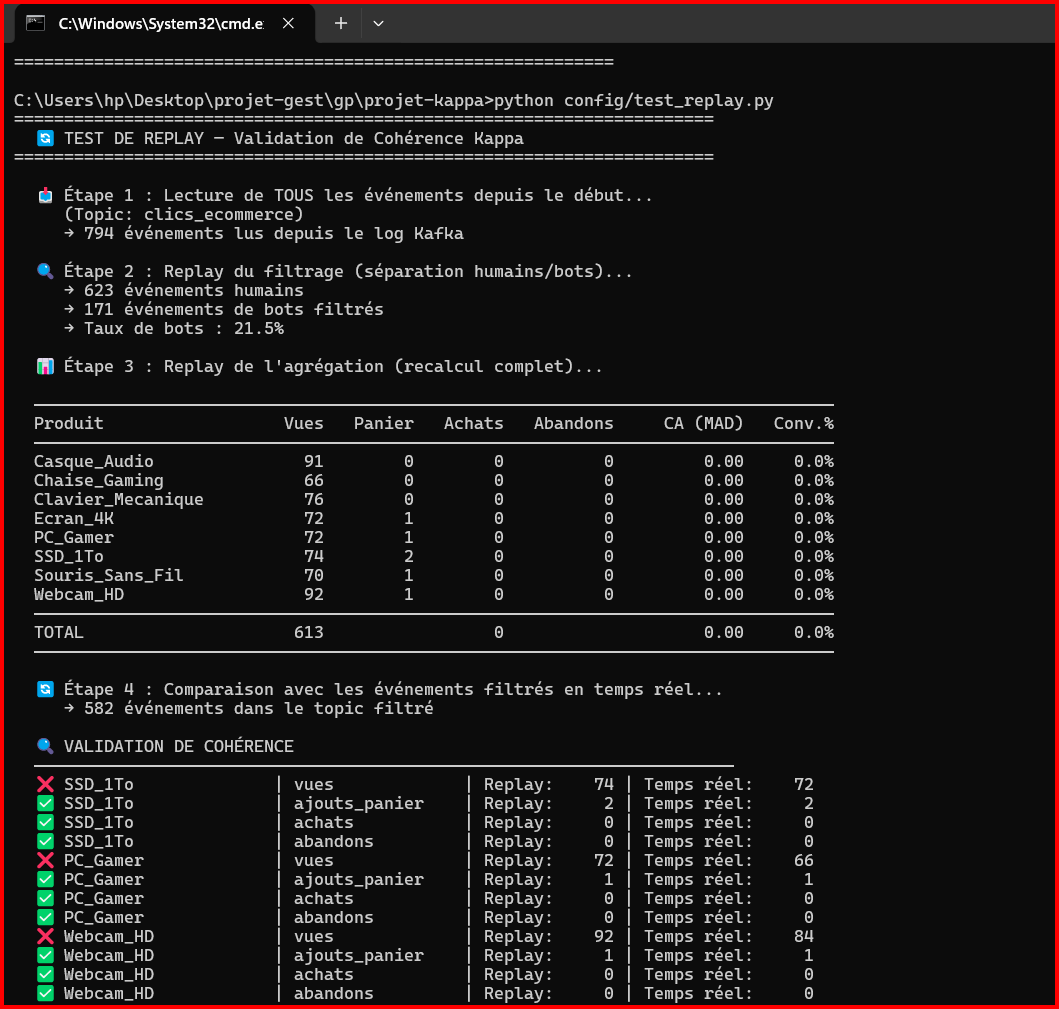
\includegraphics[width=0.78\textwidth]{../screenshots/validation_replay1.png}

  \vspace{0.3cm}
  \small C'est ce mécanisme de \textbf{replay} qui remplace le Batch Layer de Lambda.
\end{frame}

% ════════════════════════════════════════════════════════════════════════════
%  SECTION 7 — RISQUES
% ════════════════════════════════════════════════════════════════════════════
\section{Gestion des Risques}

\begin{frame}{Matrice des risques}
  \footnotesize
  \begin{tabular}{L{3.2cm} C{1.5cm} C{1.5cm} L{4.5cm} C{1cm}}
    \toprule
    \textbf{Risque} & \textbf{Prob.} & \textbf{Impact} & \textbf{Action préventive} & \textbf{Statut} \\
    \midrule
    Perte de données Kafka & \textcolor{orange}{Moy.} & \textcolor{kappaRed}{Élevé} & Rétention 7j + mécanisme replay & \textcolor{kappaGreen}{\faCheck} \\[4pt]
    Retard de livraison & \textcolor{kappaRed}{Élevée} & \textcolor{kappaRed}{Élevé} & Planning Poker + Sprints courts & \textcolor{kappaGreen}{\faCheck} \\[4pt]
    Versions incompatibles & \textcolor{orange}{Moy.} & \textcolor{kappaRed}{Élevé} & Versions figées dans Docker & \textcolor{kappaGreen}{\faCheck} \\[4pt]
    Incohérence données & \textcolor{kappaGreen}{Faible} & \textcolor{kappaRed}{Élevé} & Test de replay automatisé & \textcolor{kappaGreen}{\faCheck} \\[4pt]
    Manque compétences & \textcolor{kappaRed}{Élevée} & \textcolor{orange}{Moyen} & Formation + documentation & \textcolor{kappaGreen}{\faCheck} \\
    \bottomrule
  \end{tabular}

  \vspace{0.4cm}
  \begin{block}{Cône d'incertitude (Chapitre 8 du cours)}
    \small Au début du projet, l'incertitude liée à Kafka/Flink était très forte ($\times 4$). Après chaque Sprint, la maîtrise technique s'est améliorée et l'incertitude s'est réduite ($\times 1$).
  \end{block}
\end{frame}

\begin{frame}{Suivi des risques par Sprint}
  \centering\footnotesize
  \begin{tabular}{L{4cm} C{2.5cm} C{2.5cm} C{2.5cm}}
    \toprule
    \textbf{Risque} & \textbf{Sprint 1} & \textbf{Sprint 2} & \textbf{Sprint 3} \\
    \midrule
    R1 — Perte de données & \textcolor{orange}{Non traité} & \textcolor{kappaGreen}{Rétention config.} & \textcolor{kappaGreen}{\faCheck\ Validé} \\[4pt]
    R2 — Latence & \textcolor{kappaGreen}{Pas de problème} & \textcolor{kappaGreen}{Acceptable} & \textcolor{kappaGreen}{\faCheck\ OK} \\[4pt]
    R3 — Versions & \textcolor{kappaGreen}{\faCheck\ Résolu} & \textcolor{kappaGreen}{\faCheck} & \textcolor{kappaGreen}{\faCheck} \\[4pt]
    R4 — Mémoire & \textcolor{orange}{Docker lourd} & \textcolor{kappaGreen}{Optimisé} & \textcolor{kappaGreen}{\faCheck\ OK} \\[4pt]
    R6 — Retard & \textcolor{orange}{Sprint 1 long} & \textcolor{kappaGreen}{Rattrapage} & \textcolor{kappaGreen}{\faCheck\ Livré} \\
    \bottomrule
  \end{tabular}

  \vspace{0.4cm}
  \begin{exampleblock}{}
    \centering\small
    Tous les risques identifiés ont été \textbf{mitigés ou résolus} avant la livraison finale.
  \end{exampleblock}
\end{frame}

% ════════════════════════════════════════════════════════════════════════════
%  CONCLUSION
% ════════════════════════════════════════════════════════════════════════════
\section{Conclusion et Perspectives}

\begin{frame}{Bilan et perspectives}
  \begin{columns}[T]
    \begin{column}{0.48\textwidth}
      \begin{exampleblock}{\faCheckCircle\ Ce que nous avons accompli}
        \small
        \begin{itemize}
          \item Infrastructure Kafka/Flink/Docker
          \item Simulateur e-commerce réaliste
          \item 3 topologies de traitement de flux
          \item Rétention configurable par topic
          \item Validation de cohérence par replay
          \item Documentation complète (7 blocs)
        \end{itemize}
      \end{exampleblock}
    \end{column}
    \begin{column}{0.48\textwidth}
      \begin{block}{\faRocket\ Perspectives}
        \small
        \begin{itemize}
          \item Machine Learning en temps réel
          \item Prédiction du prochain achat
          \item Dashboard de monitoring live
          \item Déploiement cloud (AWS/GCP)
          \item Ajustement dynamique des prix
        \end{itemize}
      \end{block}
    \end{column}
  \end{columns}

  \vspace{0.5cm}
  \begin{block}{}
    \centering
    \textbf{L'architecture Kappa} a permis de traiter et d'analyser le comportement client en \textbf{temps réel} avec une parfaite \textbf{cohérence} grâce au mécanisme de rétention et de replay.
  \end{block}
\end{frame}

% ╔══════════════════════════════════════════════════════════════════════════╗
% ║  SLIDE FINALE                                                          ║
% ╚══════════════════════════════════════════════════════════════════════════╝
\begin{frame}[plain]
  \centering
  \vspace{2cm}

  {\Huge\textcolor{kappaBlue}{\textbf{Merci !}}}

  \vspace{0.8cm}
  {\Large\textcolor{kappaGold}{Des questions~?}}

  \vspace{1.5cm}
  {\small
    \textbf{Yazid TAHIRI ALAOUI} · \textbf{Souhayla ECH-CHARAY} · \textbf{Ouissal EL AMRANI}\\[6pt]
    Gestion de Projets Informatiques — Pr. Redouan ABAKOUY\\
    ENSA Al Hoceima — 2025/2026
  }

  \vspace{0.5cm}
  
\includegraphics[height=0.8cm]{logos/UAE.png}\hspace{1.5cm}%
  
\includegraphics[height=0.8cm]{logos/ENSAH.png}
\end{frame}

\end{document}
